\chapter{\IfLanguageName{dutch}{Proof of Concept}{Proof of Concept}}%
\label{ch:PoC}

Dit deel van het onderzoek presenteert een Proof of Concept gericht op welk framework er gebruikt zal worden om Machine Learning pipelines lokaal uit te voeren, en dat gebruikt kan worden in het opleidingsonderdeel Machine Learning Operations.
Het doel van deze Proof of Concept is om de efficiëntie en bruikbaarheid van deze frameworks te onderzoeken aan de hand van een lokale opstelling met de gekozen frameworks. Hierbij zullen de uitvoeringen van het framework, alsook de resultaten en bevindingen besproken worden.
Hierna wordt aan de hand van de resultaten een conclusie getrokken over het gekozen framework.

% TODO: misschien ook vermelden voor welke frameworks je een PoC hebt uitgewerkt?

\section{Vereisten}

Voordat we kunnen beginnen met het uitwerken van de volgende Proof of Concepts is bepaalde software nodig nodig op het systeem. De vereiste software omvat:

\begin{itemize}
    \item Python\footnote{\url{https://www.python.org/downloads/}}
    \item De package manager \texttt{pip}\footnote{\url{https://pip.pypa.io/en/stable/installation/}}
\end{itemize}

Deze vereisten zorgen ervoor dat de code uit de volgende secties zonder problemen werkt. Als hardwarevereisten is het voldoende om te voldoen aan de minimale vereisten van de opleiding Toegepaste Informatica\footnote{\url{https://www.hogent.be/opleidingen/bachelors/toegepaste-informatica/computervereisten/}}. De Proof of Concept zal ook geen configuratiebestanden wijzigen voor de lokale opstelling. Elk framework wordt met de standaardinstellingen uitgevoerd.

\section{Ontwikkeling van de Machine Learning pipeline}

Deze sectie bespreekt de opbouw van de Machine Learning pipeline wordt besproken zodat duidelijk is hoe de pipeline uit de proof of concepts functioneert. De Machine Learning pipeline die gebruikt zal worden, is identiek aan de pipeline uit opdracht 3 van het opleidingsonderdeel Machine Learning Operations.

Deze pipeline is ontworpen om aan de hand van \textit{Image Classification} het verschil te kunnen herkennen tussen foto's van sinaasappels en appels. Deze pipeline heeft verschillende onderdelen:

\begin{itemize}
    \item \textbf{Preprocessing:} downloaden en verwerken van de afbeeldingen
    \item \textbf{Training:} trainen van het model
    \item \textbf{Evaluatie:} evalueren van het moel
\end{itemize}

De volgende secties zullen elk van deze onderdelen toelichten en de werking ervan uitleggen. De hele pipeline wordt visueel voorgesteld op Figuur~\ref{fig:Model_Flow}.

\begin{figure}
    \centering
    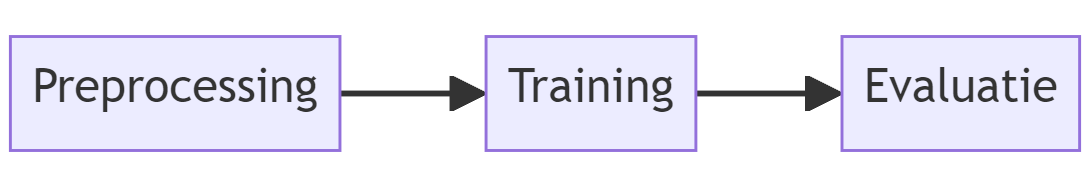
\includegraphics[width=0.9\linewidth]{graphics/Model_Diagram.PNG}
    \caption[Visuele voorstelling pipeline PoC]{Visuele voorstelling van de Machine Learning pipeline uit opdracht 3 van Machine Learning Operations}
    \label{fig:Model_Flow}
\end{figure}


\subsection{Preprocessing}

Het preprocessinggedeelte van de pipeline bereidt de afbeeldingen  zodat deze afbeeldingen gebruikt kunnen worden als invoer voor het trainen van het model. Dit omvat het downloaden en transformeren van de afbeeldingen. In deze Proof of Concept wordt gebruik gemaakt van de Tensorflow \texttt{ImageDataGenerator} om afbeeldingen in te laden, te normaliseren en te voorzien van labels gebaseerd op de mappenstructuur. Na het inladen en het klaarmaken van de afbeeldingen worden de afbeeldingen gesplitst in trainings-, validatie- en testsets. In elke van deze sets worden de juiste labels voorzien.

\subsection{Training}

Het trainingsgedeelte gaat daadwerkelijk een Machine Learning-model trainen. Deze Proof of Concept zal gebruikmaken van een Convolutional Neural Network (CNN) met behulp van Keras. Dit model bevat verschillende lagen en parameters. Er wordt gebruikgemaakt van een sequentieel model van Keras, wat betekent dat alle lagen achtereenvolgens worden uitgevoerd. De volgorde en de lagen die gebruikt worden voor dit Proof of Concept zijn als volgt:

\begin{itemize}
    \item Convolutionele laag (\texttt{Conv2D})
    \item Activatielaag (\texttt{Activation})
    \item Flatten-laag
    \item Dense-laag
\end{itemize}

\subsection{Evaluatie}

Het evaluatiegedeelte zal het getrainde model evalueren. Alle resultaten worden bijgehouden met behulp van MLFlow. De resultaten bevatten:

\begin{itemize}
    \item Parameters van het model
    \item Systeemeigenschappen en performantie
    \item Accuraatheid van het model en de evaluatie
\end{itemize}

\section{Packages}

Deze Proof of Concept maakt gebruik van verschillende packages om de Machine Learning pipeline te ontwikkelen. Deze packages zijn grotendeels dezelfde voor elke Proof of Concept, maar kunnen extra packages hebben in verband met het gekozen framework. Deze sectie behandelt alle packages die gedeeld zijn over alle Proof of Concepts.

De basispackages die gebruikt zullen worden in alle Proof of Concepts zijn:

\begin{itemize}
    \item \textbf{os:} Voor het maken van mappen voor de verschillende datasets die worden gebruikt tijdens de training en de evaluatie van het model.
    \item \textbf{Requests:} Voor het maken van HTTP-verzoeken om de nodige afbeeldingen te kunnen downloaden.
    \item \textbf{Tensorflow:} Voor het trainen en evalueren van het model, Tensorflow werkt hiervoor samen met Keras.
    \item \textbf{Keras:} Voor het maken van het model bestaande uit verschillende lagen.
    \item \textbf{MLFlow:} Voor het bijhouden van alle resultaten van het model, het trainingsproces en de evaluatie.
    \item \textbf{venv:} Voor het opzetten van virtuele Python omgevingen.
\end{itemize}

% TODO: plaats een link in een voetnoot naar de GitHub-repository van deze PoC: \footnote{\url{...}} + is het niet simpelweg de repo van de BP?

In de GitHub-repository van deze Proof of Concept zal voor elk framework een bestand genaamd \texttt{requirements\_framework.txt} te vinden zijn, waarbij `framework' de naam is van het gebruikte framework. Dit bestand kan samen met \texttt{pip} gebruikt worden om alle packages te installeren:

\begin{minted}[breaklines]{bash}
pip install -r "requirements_framework.txt"
\end{minted}

\subsection{Virtuele omgeving}

De volgende secties zullen gebruikmaken van verschillende frameworks. Deze frameworks hebben allemaal de mogelijkheid om lokaal een Machine Learning pipeline uit te voeren en voldoen ook aan alle must haves uit de requirementsanalyse (zie Sectie~\ref{s:Requirementsanalyse}).

Voor elk gebruikt framework wordt een virtuele omgeving opgesteld. Dit zorgt ervoor dat er geen conflicten zijn tussen de verschillende versies van de libraries.

Om gebruik te maken van de virtuele omgeving van de Proof of Concept moet het volgene commando uitgevoerd worden:

\begin{minted}[breaklines]{bash}
    .\dagster\Scripts\activate
\end{minted}

Dit zal de virtuele omgeving opstarten in de console waar het commando is uitgevoerd. Elk commando dat nu in deze terminal wordt uitgevoerd, gebeurt binnen de virtuele omgeving.


\section{MLflow}

Elk van de Proof of Concepts bevat MLflow. Zoals besproken in Sectie~\ref{subsec:mlflow} heeft dit framework veel functionaliteiten. Voor deze Proof of Concepts worden vooral de parameters van het model, de resultaten van de training en de resultaten van de evaluatie bijgehouden. Dit wordt \textit{Experiment Tracking} genoemd en maakt het mogelijk om experimenten bij te houden.

\subsection{Installatie}

Alvorens MLFlow gebruikt kan worden, moet het geïnstalleerd worden. Dit kan met behulp van \texttt{pip}:

\begin{minted}{bash}
    pip install MLFlow
\end{minted}

Vervolgens kan MLFlow geïmporteerd worden in de Python-code:

\begin{minted}{python}
    import mlflow
    import mlflow.keras
\end{minted}

Nadat MLflow geïmporteerd is, moeten alle parameters in de code aangepast worden. Zo stuurt het de resultaten naar de juiste server en worden de juiste resultaten bijgehouden. De parameters die aangepast moeten worden zijn als volgt:

\begin{itemize}
    \item \textbf{Parameter Logging}: Het commando hiervoor is \texttt{mflow().log\_param}. Dit houdt alle parameters van het model bij, zoals het aantal epochs of de batchgrootte.
    \item \textbf{Metric Logging}: Tijdens het trainen van het model zal MLflow belangerijke resulaten bijhouden, zoals de nauwkeurigheid en het verlies van het model. Dit word aan de hand van \texttt{mlflow.log\_metric()} bijgehouden. Deze metrics worden voor elke epoch van het trainingsproces bijgehouden om het verloop van de training te analyseren.
\end{itemize}

Als MLflow geinstalleerd is en alle parameters correct zijn ingesteld, kan de lokale server worden opgestart met het volgende commando:

\begin{minted}{bash}
    mlflow server --host 127.0.0.1 --port 8080
\end{minted}

Dit commando heeft de volgende parameters:

\begin{itemize}
    \item \texttt{host}: voor het instellen van het ip addres voor de lokale server.
    \item \texttt{port}: voor het instellen van de poort van de lokale server.
\end{itemize}

Nadat de server opgestart is, kan naar het ingestelde adres worden genavigeerd in een webbrowser om het dashboard te zien. Het dashboard van MLflow toont de resulaten van alle pipelines weer, zie het voorbeeld in Figuur~\ref{fig:mlflow_dashboard}.

\begin{figure}
    \centering
    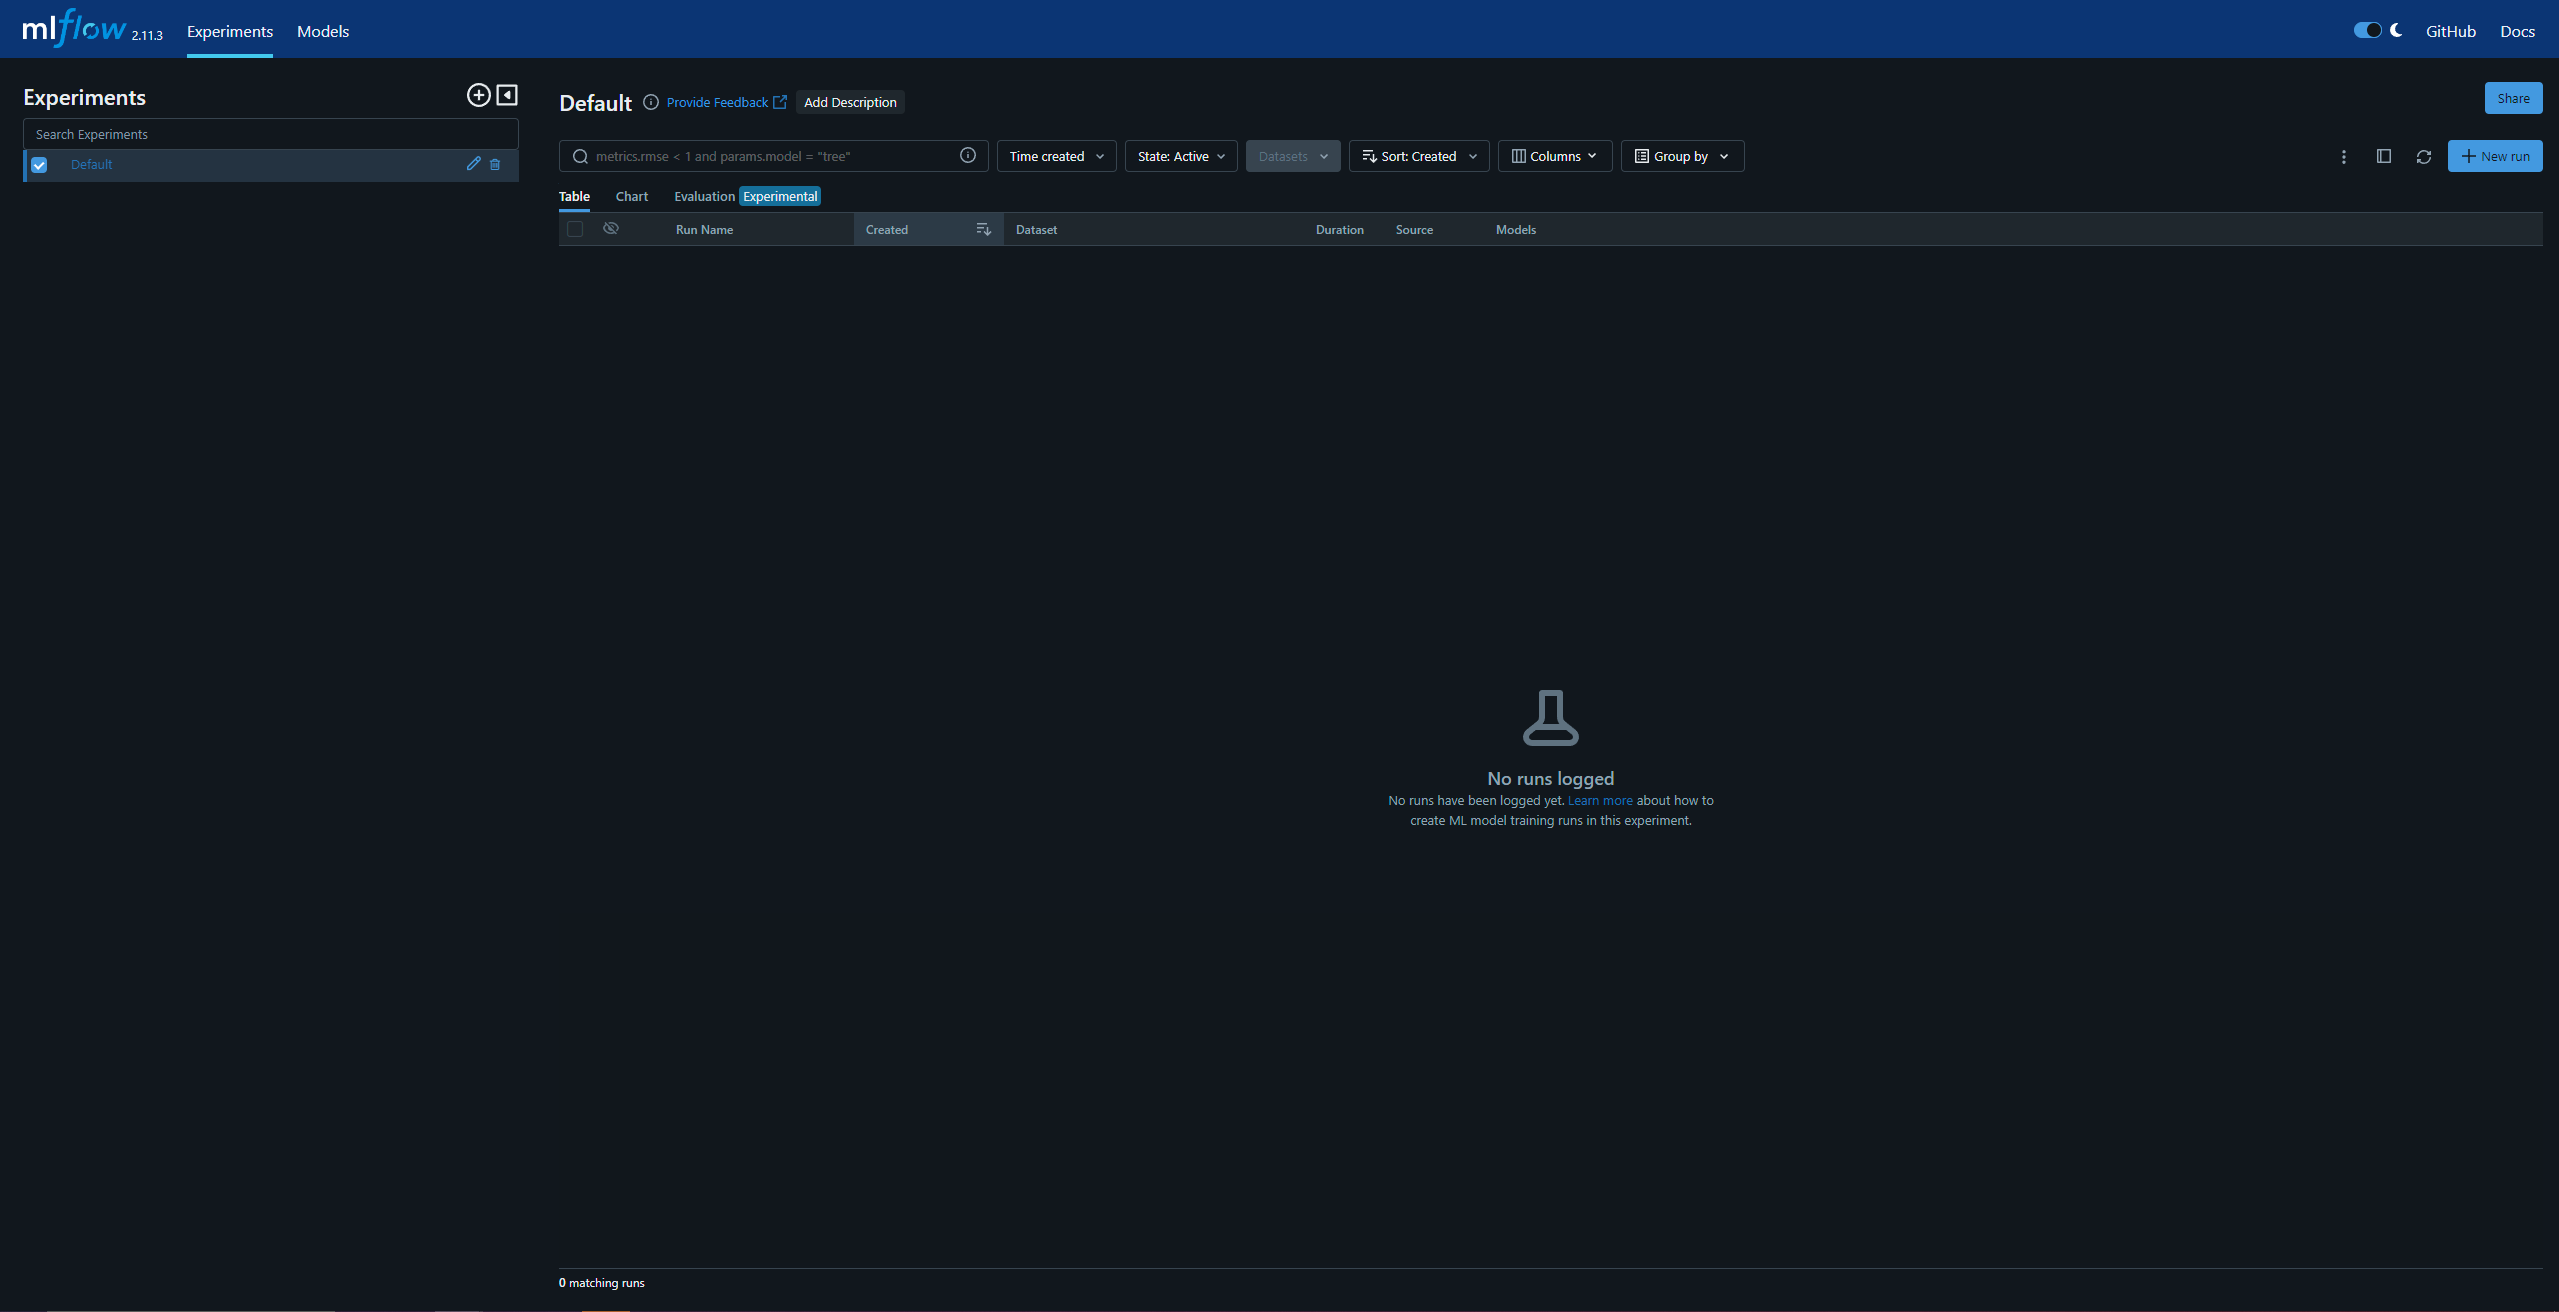
\includegraphics[width=0.9\linewidth]{graphics/mlflow_dashboard.PNG}
    \caption{Voorbeeld van het MLflow dashboard}
    \label{fig:mlflow_dashboard}
\end{figure}

\section{Prefect}

Een eerste tool waarvan een Proof of Concept gemaakt wordt is Prefect. Dit zal, in combinatie met MLFlow, gebruikt worden voor het lokaal uitvoeren van Machine Learning pipelines. Hierbij worden alle aanpassingen in de code van het framework vergeleken met de originele code van opdracht 3 van opleidingsonderdeel Machine Learning Operations.

\subsection{Installatie}

De installatie van Prefect gebeurt met de package manager \texttt{pip}. Via de terminal kan Prefect met het volgende commando geïnstalleerd worden, dit zal ook alle benodigde packages installeren:


\begin{minted}{bash}
    pip install -r "requirements_Prefect.txt"
\end{minted}

Om alleen Prefect te installeren kan dit met het volgende \texttt{pip} commando:

\begin{minted}{bash}
    pip install prefect
\end{minted}

\subsection{Lokale Server}

Prefect heeft de mogelijkheid om Machine Learning pipelines lokaal uit te voeren, dit gebeurt met behulp van een lokale server. Deze server kan worden opgestart met het commando:

\begin{minted}{bash}
    prefect server start
\end{minted}

Na het uitvoeren van het startcommando zou het resultaat van Figuur~\ref{fig:Prefect_server} te zien moeten zijn.
\begin{figure}
    \centering
    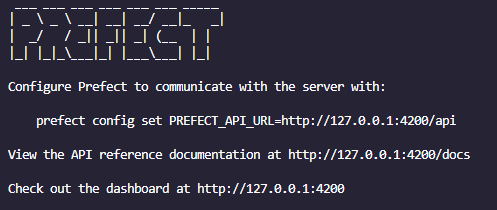
\includegraphics[width=0.9\linewidth]{graphics/Prefect_server.PNG}
    \caption{Uitvoer van de Prefect Server}
    \label{fig:Prefect_server}
\end{figure}

Nu de server is opgestart, moet de code nog communiceren met de Prefect webinterface. Zoals Figuur~\ref{fig:Prefect_server} aantoont, wordt dit gedaan aan de hand van een commando dat gebruikmaakt van een lokale API:

\begin{minted}{bash}
    prefect config set PREFECT_API_URL=http://127.0.0.1:4200/api
\end{minted}

Nu de server opgestart en verbonden is met de lokale omgeving, kan via de ingestelde link het Prefect dashboard worden bezocht.

\subsection{Dashboard}

Het dashboard van Prefect is een omgeving waarin alle pipeline flows worden beheerd. Figuur~\ref{fig:Prefect_Dashboard} geeft een voorbeeld van het Prefect dashboard.

\begin{figure}
    \centering
    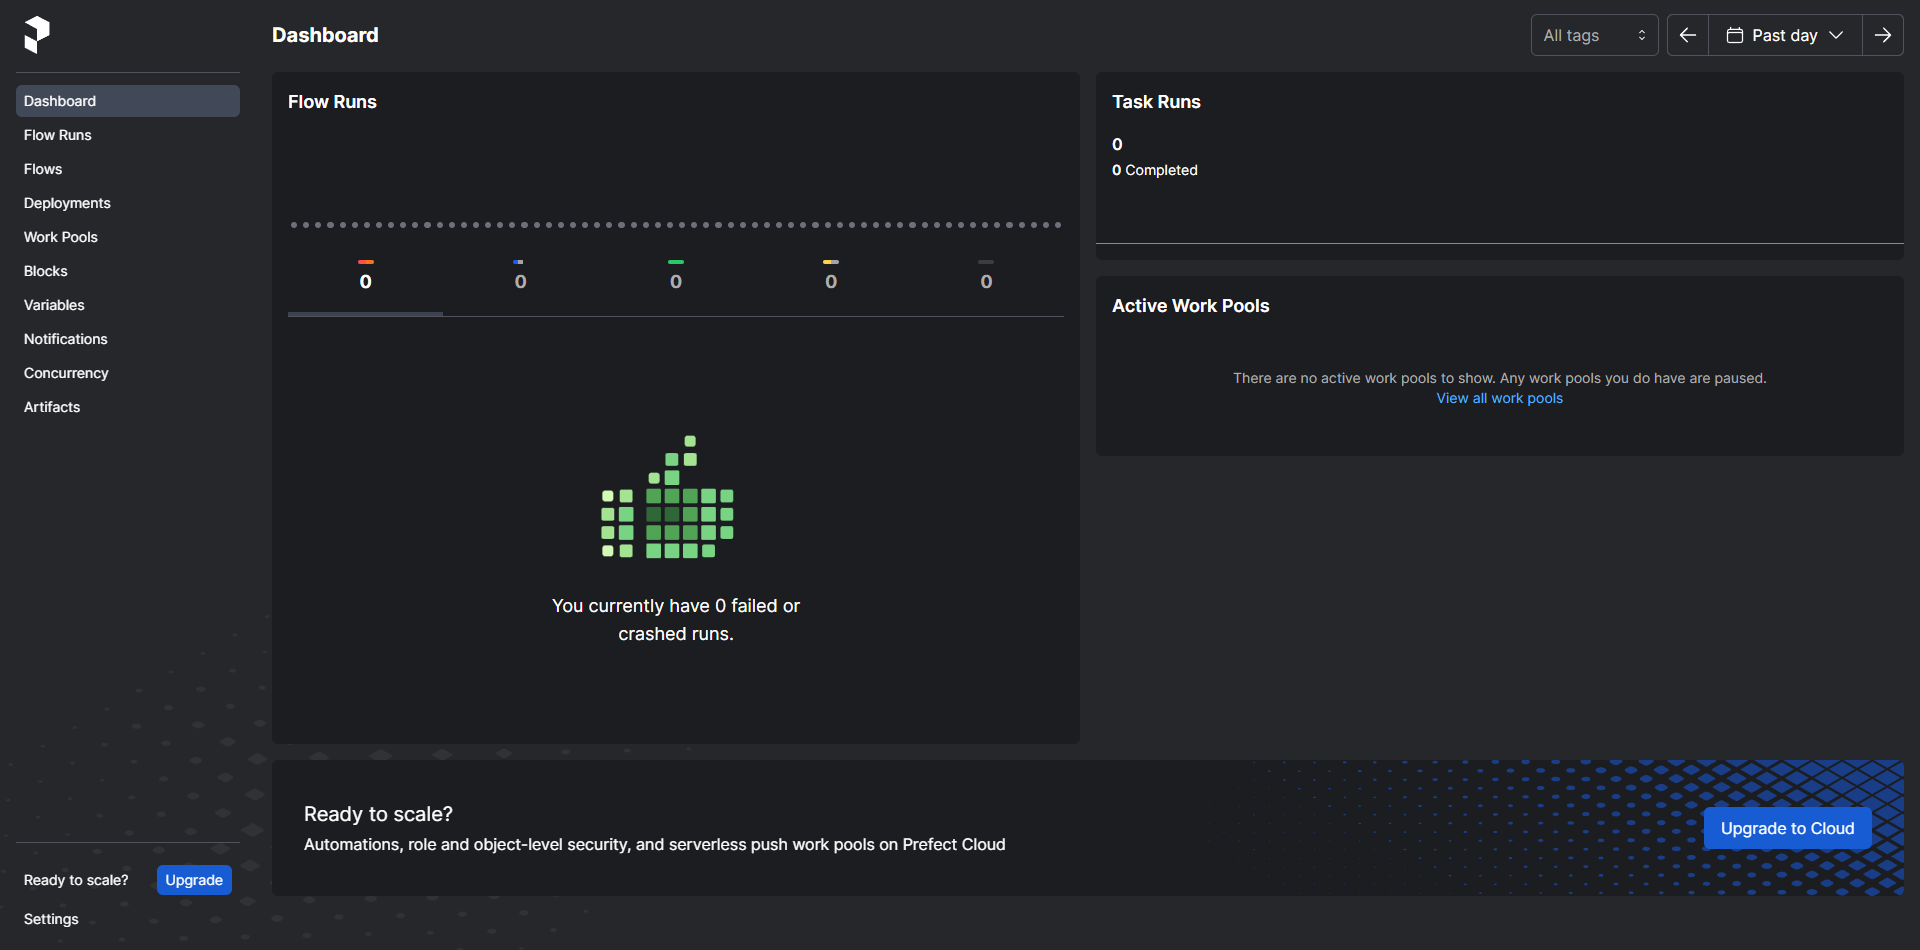
\includegraphics[width=0.9\linewidth]{graphics/Prefect_dashboard.PNG}
    \caption{Voorbeeld van het Prefect Dashboard}
    \label{fig:Prefect_Dashboard}
\end{figure}

De functies die kunnen worden gezien op Figuur~\ref{fig:Prefect_Dashboard} zijn:

\begin{itemize}
    \item \textbf{Dashboard:} Geeft een overzicht van alle flow runs. Hier kan worden bekeken wanneer een flow succesvol of onsuccesvol is uitgevoerd.
    \item \textbf{Flow Runs:} Geeft een tijdlijn weer met alle flows die uitgevoerd zijn over een bepaalde tijd.
    \item \textbf{Flows:} Toont elke flow aan die in de code is geschreven. Hierbij kan ook in de flow gekeken worden om te zien welke taken het bevat.
    \item \textbf{Deployments:} Geeft alle deployments weer. Dit zijn flows die rechtstreeks met het dashboard kunnen worden uitgevoerd.
    \item \textbf{Blocks:} Hier wordt alle gevoelige informatie bijgehouden, zoals wachtwoorden en API keys.
    \item \textbf{Work Pools:} Hier kan verbinding gemaakt worden met een cloud omgeving om de pipeline daar te laten uitvoeren.
\end{itemize}

Deze Proof of Concept zal gebruik maken van de \textit{Flow runs} en \textit{Flows} pagina's op het dashboard.

\subsection{Uitvoering}

Prefect werkt met decorators. Dit zorgt ervoor dat bestaande Python-functies eenvoudig kunnen worden omgezet naar het Prefect framework. De twee decorators \texttt{@task} en \texttt{@flow} werden eerder in de Sectie~\ref{subsec:prefect} besproken. Deze maken het mogelijk om bestaande Python functies om te zetten naar het Prefect framework.

Origineel bevatte het preprocessinggedeelte het downloaden en het verwerken van de afbeeldingen. Echter, voor het uitvoeren in Prefect werd dit nog eens onderverdeeld in twee aparte delen. Het downloaden en het verwerken van de afbeeldingen gebeurt dus apart. De volledige code van de pipeline is te vinden in de GitHub-repository van deze Proof of Concept. % TODO: refereer naar dezelfde voetnoot hier

De download functie werd een \texttt{Task} de andere functies werden een \texttt{Flow}. Dit werd gedaan door de decorators voor de functie te plaatsen. Uiteindelijk worden dan alle \texttt{Tasks} en \texttt{Flows} samengevoegd in één pipeline.

\subsubsection{Pipeline}

De pipeline in Prefect is een flow waarin alle taken en flows achter elkaar worden uitgevoerd. De flow of pipeline ziet er als volgt uit:

\begin{minted}[frame=lines,breaklines,linenos]{python}
@flow(task_runner=SequentialTaskRunner(), log_prints=True)
def main():
    tracking_uri = "http://127.0.0.1:8080"
    model_name = "PoC"
    mlflow.set_tracking_uri(tracking_uri)
    mlflow.set_experiment(model_name)
    download()
    preprocess()
    model = train()
    eval(model)
\end{minted}

Deze code stelt eerst het juiste tracking adres in voor MLflow, alsook de modelnaam. Hierna worden alle functies achter elkaar uitgevoerd en kunnen deze dan ook in de dashboard gezien worden.

In dit geval heeft de \texttt{@flow} nog extra parameters, deze betekenen:

\begin{itemize}
    \item \texttt{task\_runner}: Geeft aan hoe de taken en flows moeten uitgevoerd worden. In dit geval is dat een \texttt{SequentialTaskRunner} wat betekent dat alle tasks en flows achter elkaar worden uitgevoerd.
    \item \texttt{log\_prints}: Geeft alle prints weer die in de Python code werden gebruikt. In dit geval is de waarde \texttt{True}. Dit maakt het debuggen eenvoudig tijden het ontwikkelen van de pipeline.
\end{itemize}

Na het uitvoeren van de flow word deze flow gevisualiseerd in de web interface van Prefect. Figuur~\ref{fig:Prefect_Flow} toont hoe deze pagina in Prefect eruit ziet.
\begin{figure}
    \centering
    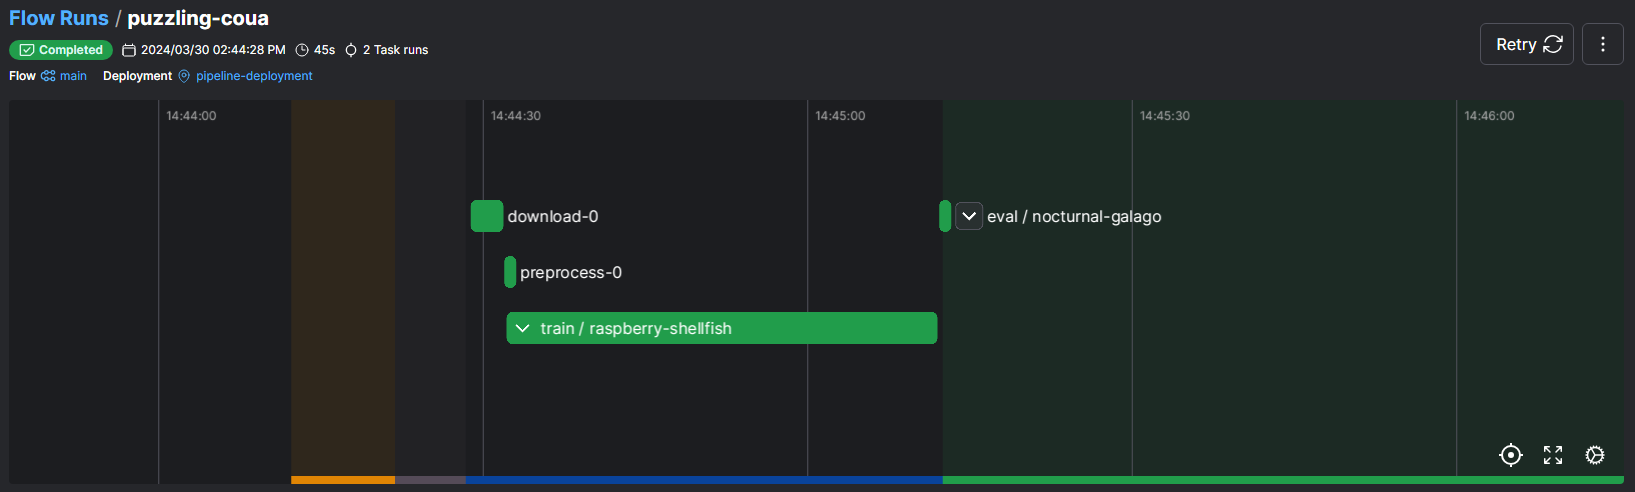
\includegraphics[width=0.9\linewidth]{graphics/Prefect_Flow.PNG}
    \caption{Flow gevisualiseerd in Prefect}
    \label{fig:Prefect_Flow}
\end{figure}

\subsection{Problemen}

Prefect had moeite met het doorgeven van parameters naar de volgende task, waardoor de flow niet meer kon werken. Om dit op te lossen werd er gebruik gemaakt van een subflow. Subflows zijn flows die worden uitgevoerd in een bestaande flow. Deze ontvangen wel goed de parameters en kunnen alles goed uitvoeren.

\subsection{Cloud}

Prefect heeft een concept genaamd \textit{Work Pools}. Figuur~\ref{fig:Prefect_Work_Pools} toont hoe deze pagina in Prefect eruit ziet.

\begin{figure}
    \centering
    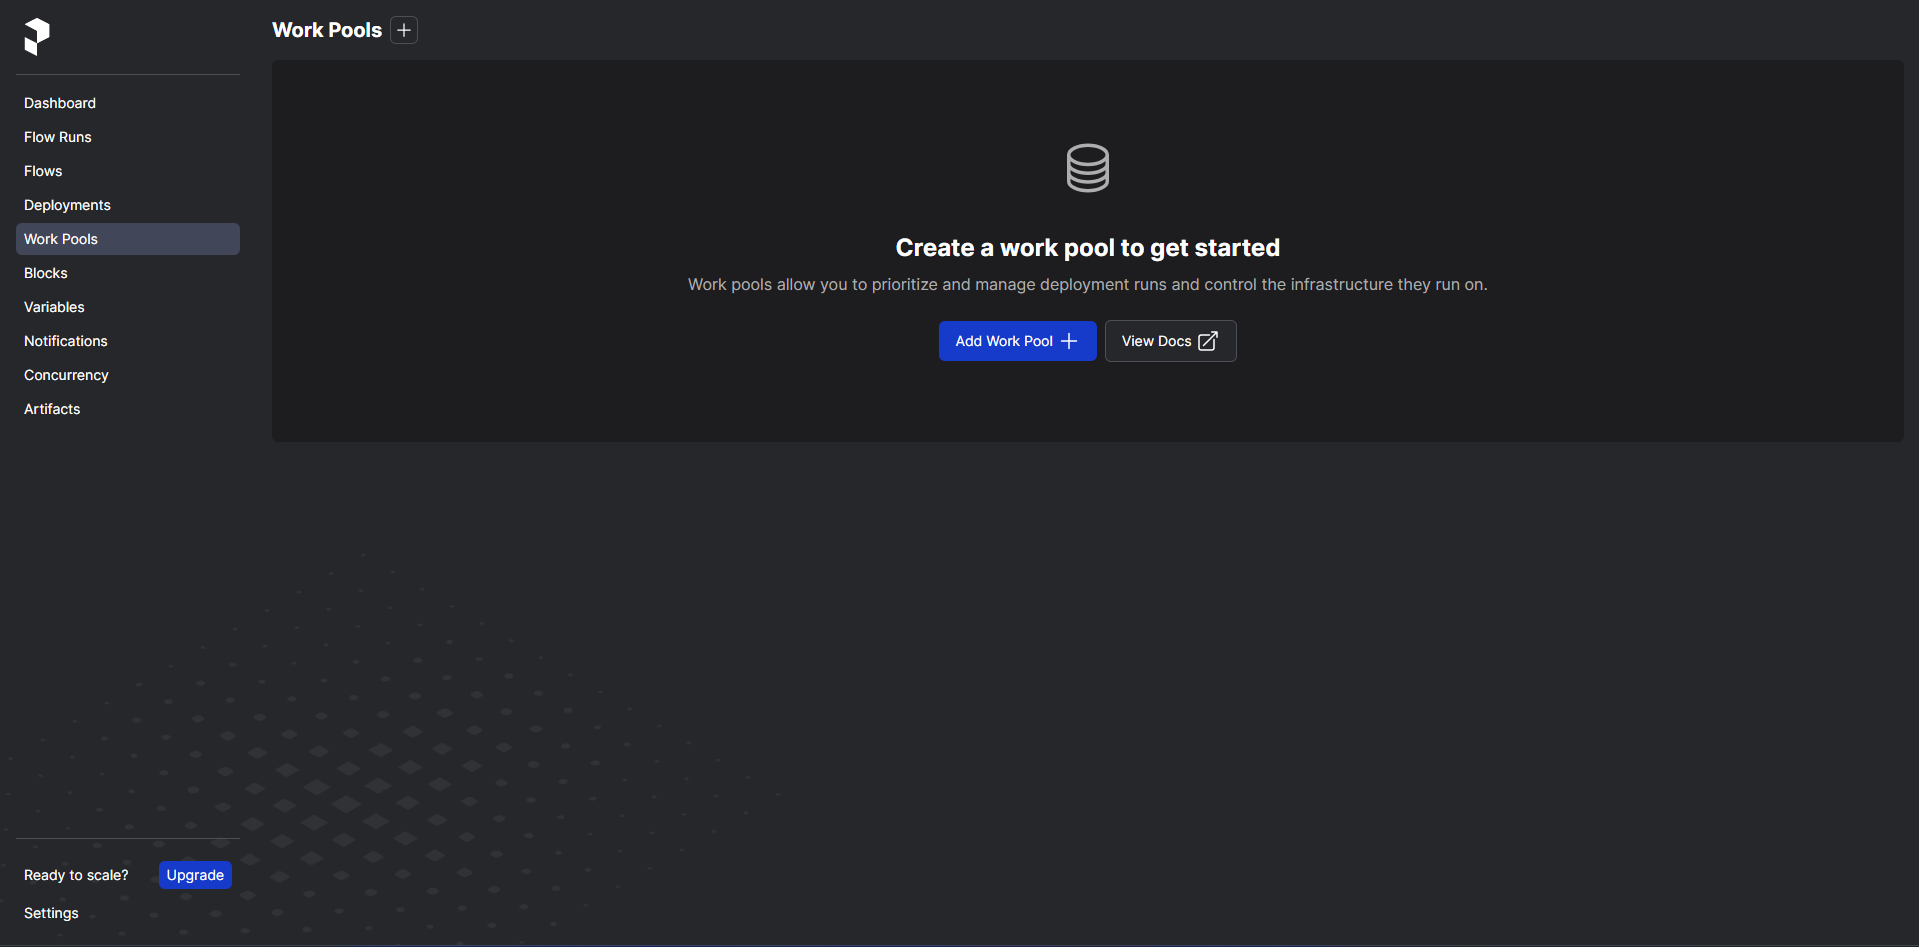
\includegraphics[width=0.9\linewidth]{graphics/Prefect_Work_Pools.PNG}
    \caption{Voorbeeld van de Prefect Work Pool pagina}
    \label{fig:Prefect_Work_Pools}
\end{figure}

Op deze pagina kan er een work pool worden toegevoegd. Dit zorgt voor een verbinding met een cloud omgeving, zodat de Prefect flow in de cloud kan worden uitgevoerd. Het aanmaken van een verbinding kan via de knop \texttt{Add Work Pool}, zoals te zien is op Figuur~\ref{fig:Prefect_Work_Pools}.

Na het klikken op deze knop kan de gewenste cloudomgeving gekozen worden (zie Figuur~\ref{fig:Prefect_Work_Pools_Create}).

\begin{figure}
    \centering
    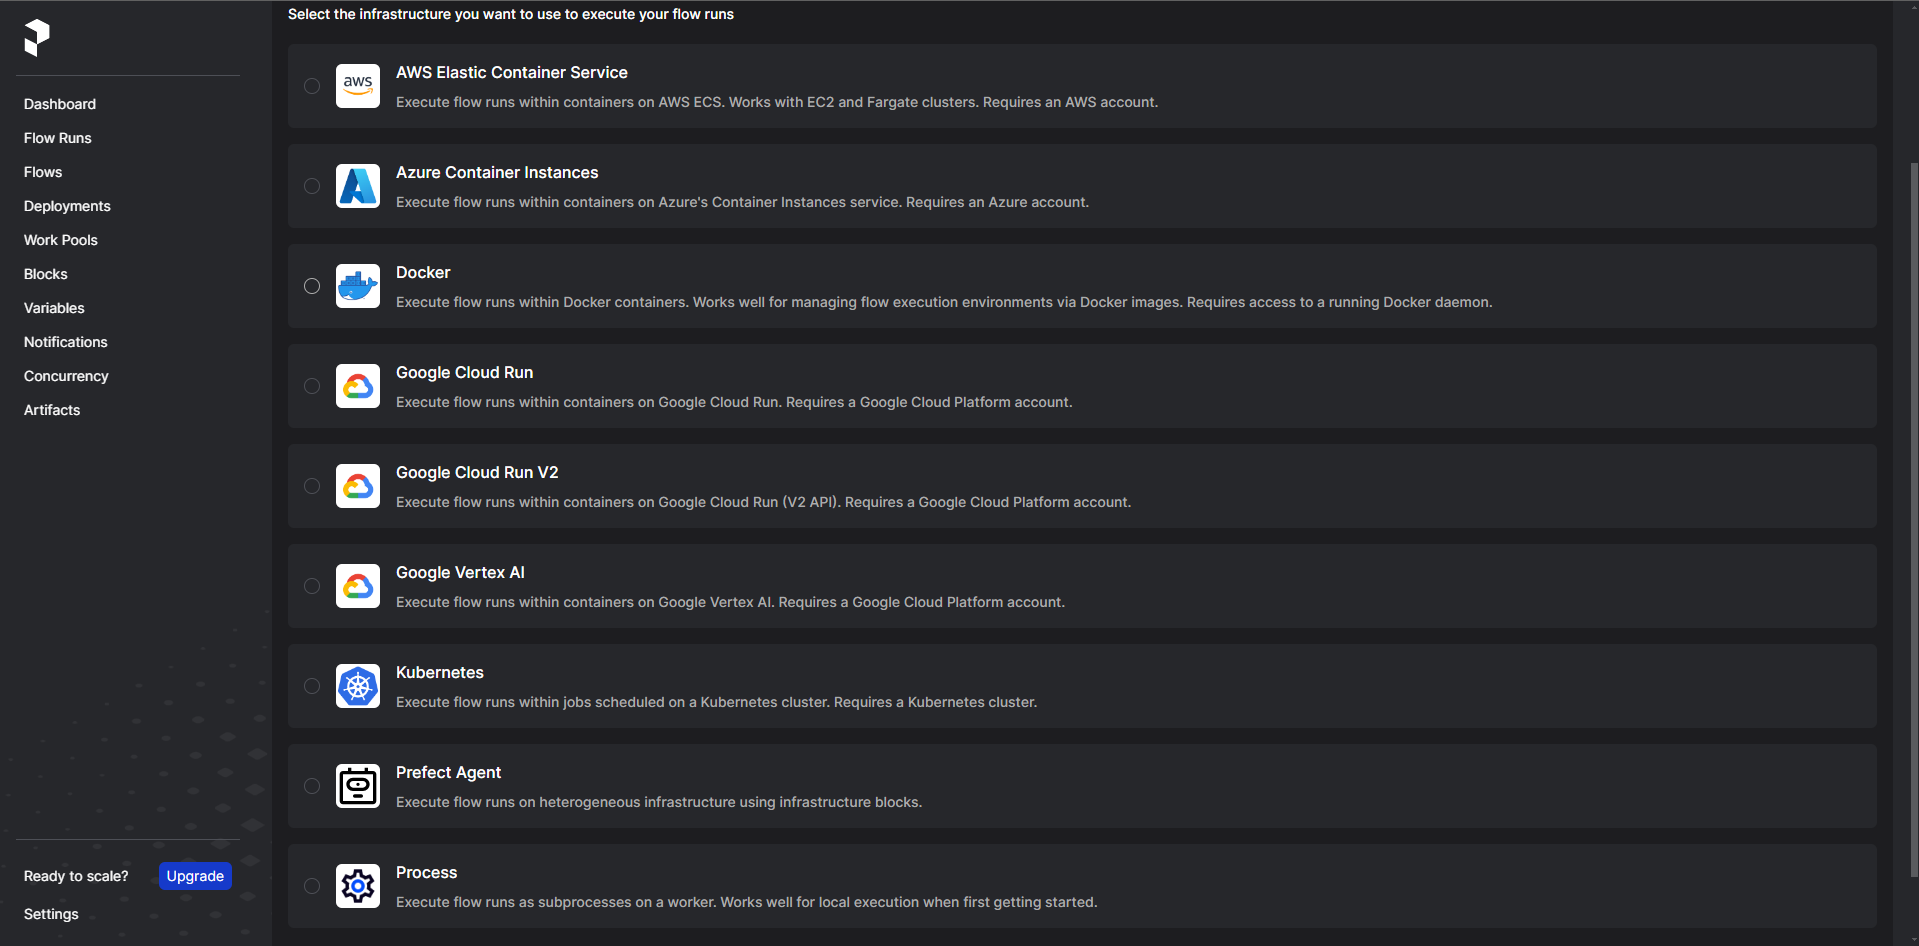
\includegraphics[width=0.9\linewidth]{graphics/Prefect_Work_Pools_Create.PNG}
    \caption{Mogelijke cloud omgevingen voor Prefect Work Pools}
    \label{fig:Prefect_Work_Pools_Create}
\end{figure}

Figuur~\ref{fig:Prefect_Work_Pools_Create} toont de verschillende cloud omgevingen waarmee Prefect kan werken. Deze omvatten onder andere AWS Elastic Container Service, Azure Container Instances, Docker, Google Cloud Run (v2), Google Vertex AI, Kubernetes, Prefect Agent en Process.

In dit voorbeeld wordt \texttt{Process} geselecteerd omdat er momenteel geen toegang is tot een cloudomgeving. De volgende stap is het invullen van details. Deze details zijn de naam en de beschrijving van de work pool en eventuele concurrency. Alleen de naam is verplicht in te vullen, zoals te zien is op Figuur~\ref{fig:Prefect_Work_Pools_Create_Details}.

\begin{figure}
    \centering
    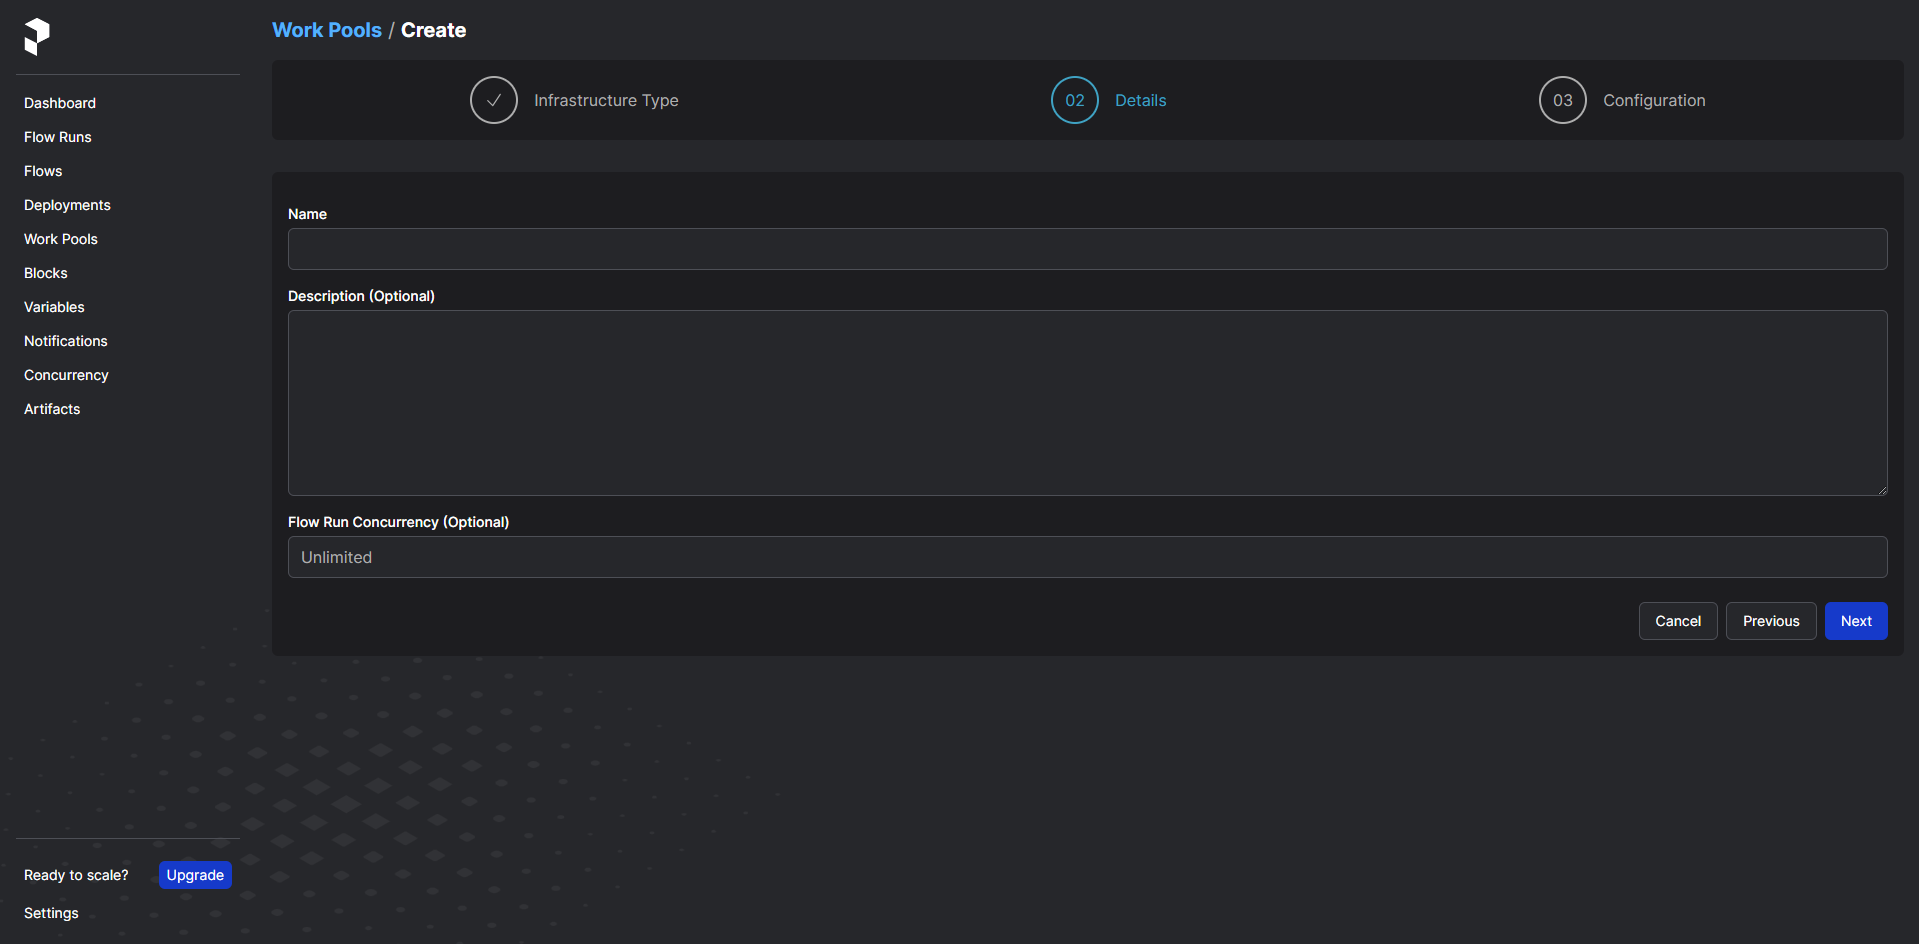
\includegraphics[width=0.9\linewidth]{graphics/Prefect_Work_Pools_Create_Details.PNG}
    \caption{Details van de create van een Prefect Work Pool}
    \label{fig:Prefect_Work_Pools_Create_Details}
\end{figure}

Op de laatste pagina worden ten slotte extra parameters ingesteld met betrekking tot de cloudprovider, zoals te zien is op Figuur~\ref{fig:Prefect_Work_Pools_Create_parameters}

\begin{figure}
    \centering
    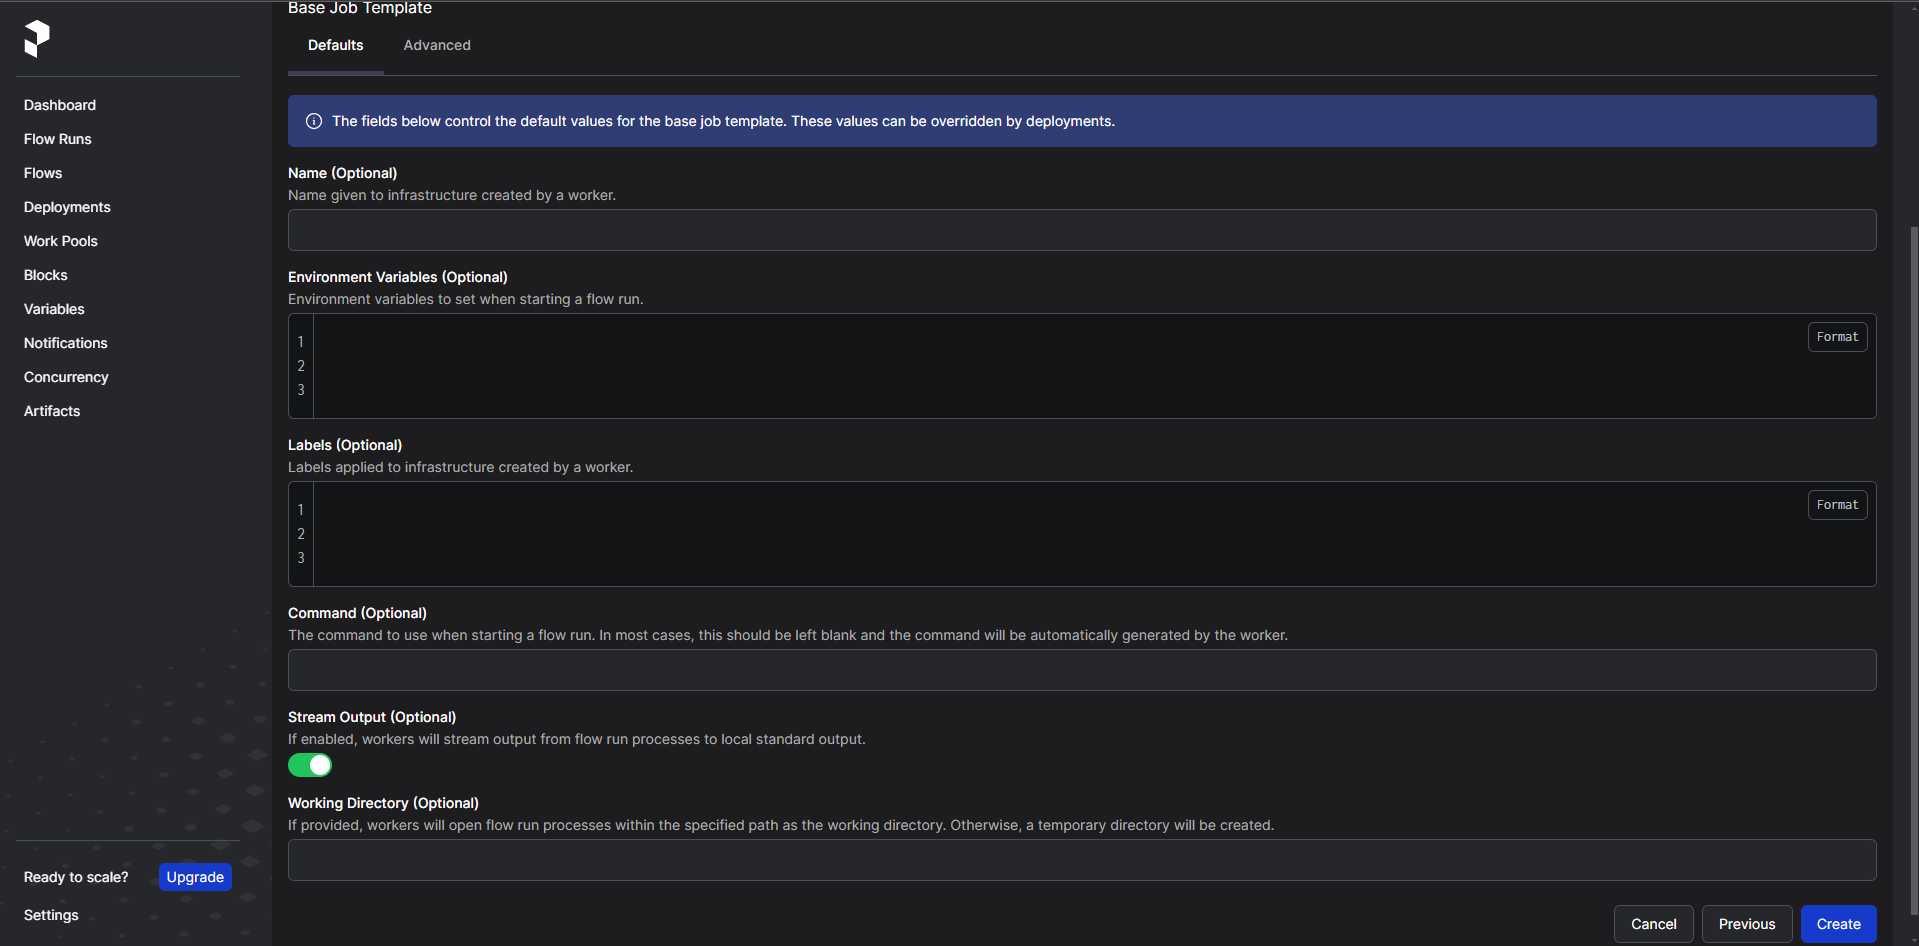
\includegraphics[width=0.9\linewidth]{graphics/Prefect_Work_Pools_Create_Parameters.PNG}
    \caption{Prefect Work Pool Creation Details}
    \label{fig:Prefect_Work_Pools_Create_parameters}
\end{figure}
\section{ZenML}
\subsection{Installatie}
De installatie van ZenML is via de package manager \texttt{pip} en kan met het volgende commando geïnstalleerd worden.
\begin{minted}[frame=lines,breaklines,linenos]{bash}
    pip install zenml
\end{minted}
Er moet wel rekening gehouden worden dat ZenML alleen werk met de Python versies 3.8, 3.9, 3.10 en 3.11.
Voor het lokaal uitvoeren van het ZenML dashboard moet er ook nog een extra package geïnstalleerd worden:
\begin{minted}[frame=lines,breaklines,linenos]{bash}
    pip install "zenml[server]"
\end{minted}

Nu dat de server geïnstalleerd is kan deze worden opgestart met het volgende commando: 
\begin{minted}{bash}
    zenml up --blocking
\end{minted}
Er wordt een extra parameter \texttt{blocking} toegevoegd omdat Windows ZenML niet als achtergrondproces kan uitvoeren. Het is ook mogelijk om ZenML in een Docker-container uit te voeren met de parameter \texttt{docker}.

Na het opstarten van de server kan in de console het serveradres gevonden worden, zoals te zien is in de figuur~\ref{ZenMLServer}
\begin{figure}
    \centering
    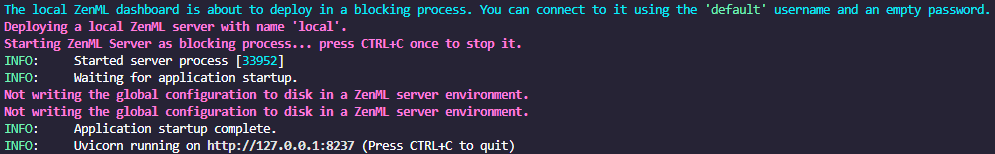
\includegraphics[width=0.9\linewidth]{graphics/ZenML_Server.PNG}
    \caption{ZenML server uitvoer na het opstarten}
    \label{fig:ZenMLServer}
\end{figure}
\subsection{Dashboard}
Wanneer er genavigeerd wordt naar het serveradres, zal er gevraagd worden om in te loggen. De inloggegevens zijn te zien bij het opstarten van de server in de console. Figuur~\ref{fig:ZenMLServer} toont dit ook aan. Hier kan gezien worden dat de gebruikersnaam \texttt{default} is en dat het wachtwoord leeg gelaten mag worden. Het inlogscherm ziet eruit zoals weergegeven in figuur~\ref{fig:ZenML_Login}
\begin{figure}
    \centering
    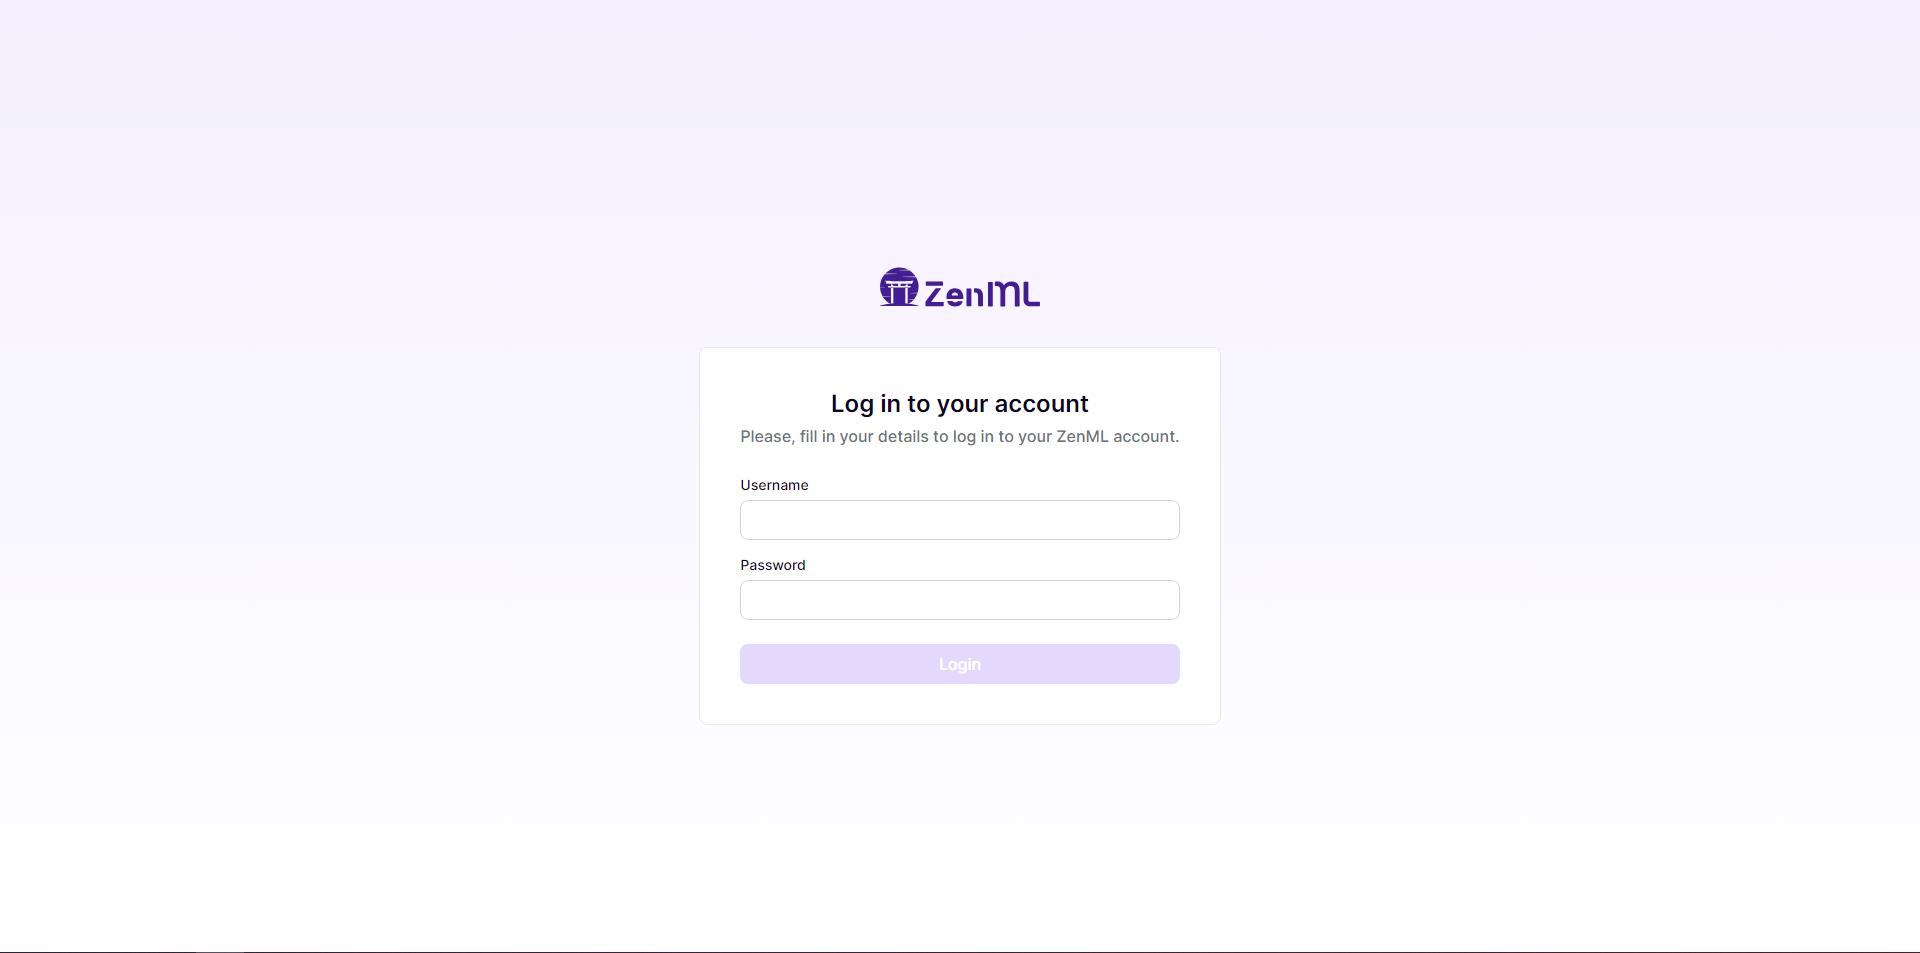
\includegraphics[width=0.9\linewidth]{graphics/ZenML_Login.PNG}
    \caption{ZenML authenticatie pagina}
    \label{fig:ZenML_Login}
\end{figure}
Na het inloggen wordt gevraagd om enkele basisgegevens, zoals je naam, e-mailadres, het gebruiksdoel van ZenML en hoe je ZenML hebt ontdekt. Het invullen van de naam en het e-mailadres is optioneel, maar de overige velden zijn verplicht.
Nu dat alles is ingevuld kan het dashboard gezien worden. Dit dashboard ziet er uit zoals op figuur~\ref{fig:ZenML_Overview}
\begin{figure}
    \centering
    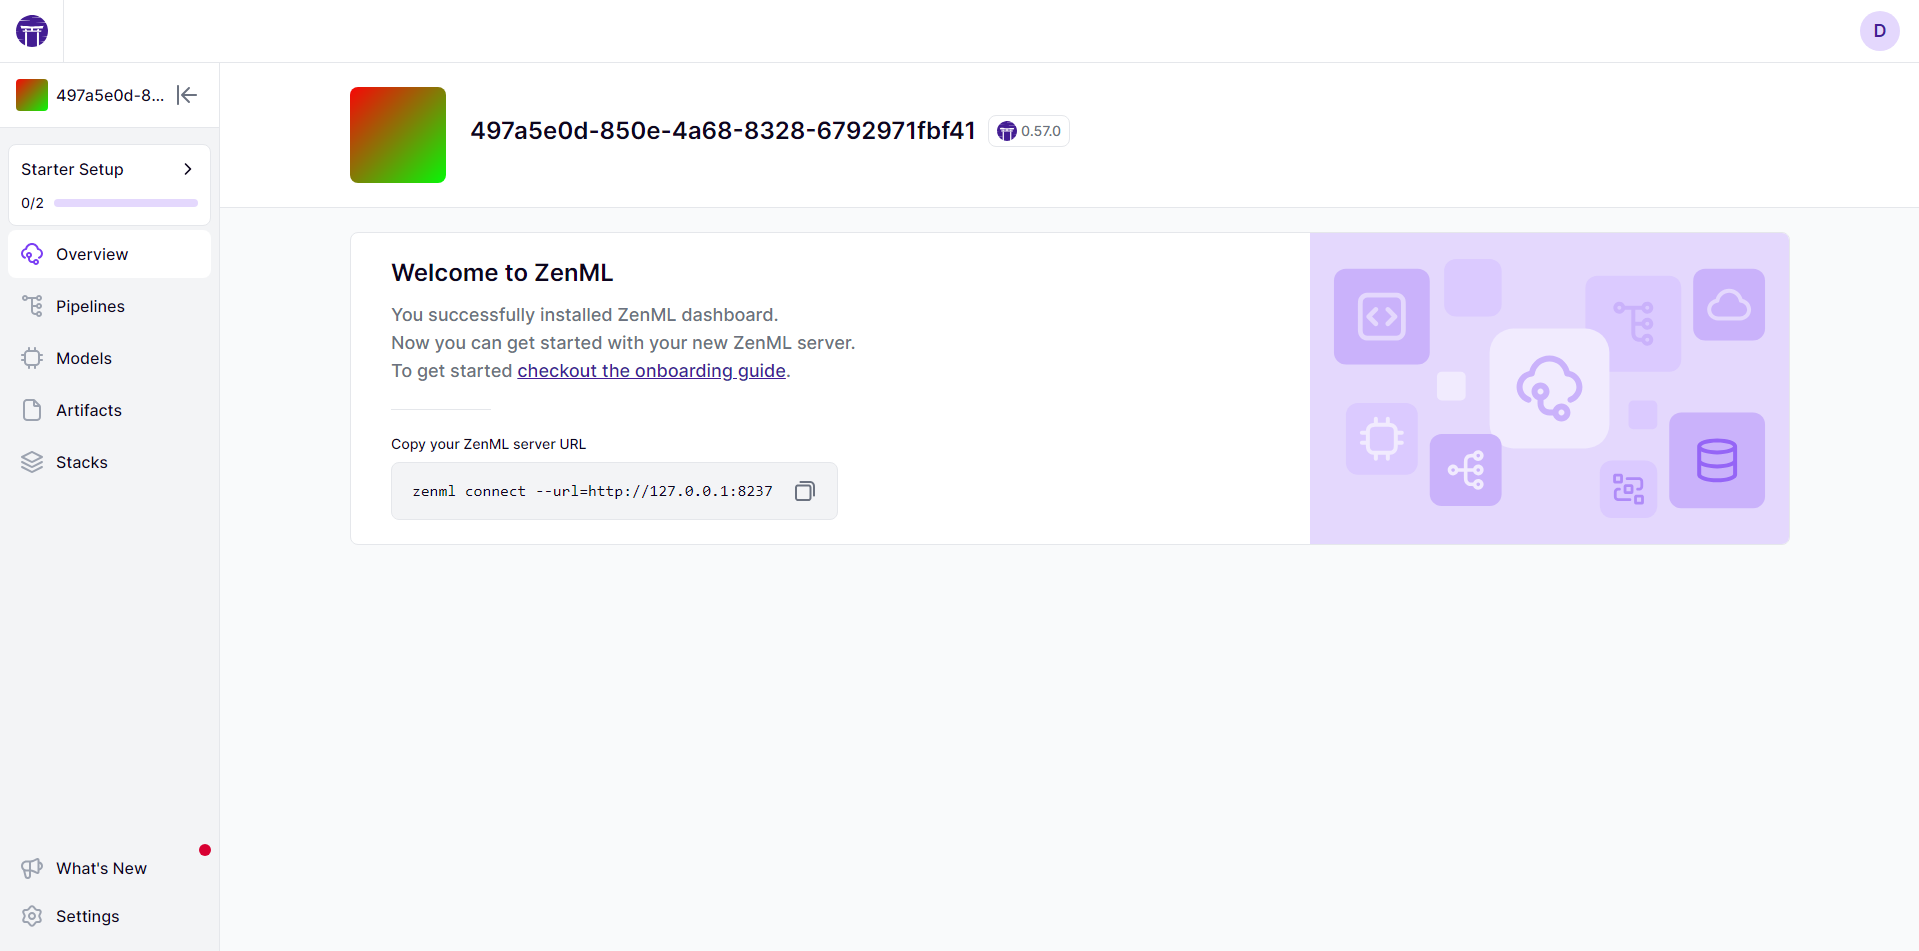
\includegraphics[width=0.9\linewidth]{graphics/ZenML_Overview.PNG}
    \caption{ZenML startpagina}
    \label{fig:ZenML_Overview}
\end{figure}
De functies die kunnen worden gezien op Figuur~\ref{fig:ZenML_Overview} zijn:

\begin{itemize}
    \item \textbf{Overview:} Geeft weer hoe je verbinding kunt maken met de ZenML-server, zodat je meerdere computers aan één server kunt koppelen.
    \item \textbf{Pipelines:} Geeft alle pipelines weer die werden of worden uitgevoerd.
    \item \textbf{Models:} Maakt het mogelijk voor het beheren van getrainde Machine Learning modellen. (Dit is een ZenML Cloud optie en is betalend)
    \item \textbf{Artifacts:} De output van het training process word hier bijgehouden. (Dit is een ZenML Cloud optie en is betalend)
    \item \textbf{Stacks:} Hier kan verbinding gemaakt worden met verschillede integraties zoals: Discord, Azure, Docker, Kubernetes, etc.
    \item \textbf{Settings:} Hier wordt alle gevoelige informatie bijgehouden, zoals wachtwoorden en API keys. Alsook GitHub-repositories.
\end{itemize}
Deze Proof of Concept zal gebruik maken van de \textit{Pipelines} pagina op het dashboard.

\subsection{Uitvoering}
ZenML werkt met decorators. Dit zorgt ervoor dat bestaande Python-functies eenvoudig kunnen worden omgezet naar het ZenML framework. De twee decorators \texttt{@step} en \texttt{@pipeline} werden eerder in de Sectie~\ref{subsec:ZenML} besproken. Deze maken het mogelijk om bestaande Python functies om te zetten naar het ZenML framework.

Origineel bevatte het preprocessingsgedeelte zowel het downloaden als het verwerken van de afbeeldingen. Voor gebruik in ZenML is dit echter opgesplitst in twee aparte stappen: het downloaden en het verwerken van de afbeeldingen gebeurt nu afzonderlijk. Ook bij het maken van het model wordt het model eerst gebouwd en pas daarna getraind. In de originele code gebeurde dit in één functie.
De volledige code van de pipeline is te vinden in de GitHub-repository{\url{https://github.com/casperaudenaert/BP}} van deze Proof of Concept. % TODO: refereer naar dezelfde voetnoot hier

Alle functies werden een \texttt{step}. Dit werd gedaan door de decorators voor de functie te plaatsen. Uiteindelijk worden dan alle \texttt{steps} samengevoegd in één pipeline dit word aan de hand van de \texttt{pipeline} decorator gedefinieerd.
\subsection{Pipeline}
De pipeline in ZenML is een functie waarin alle taken en steps achter elkaar worden uitgevoerd. De pipeline ziet er als volgt uit:
\begin{minted}[frame=lines,breaklines,linenos]{python}
@pipeline(enable_cache=False)
def main():
    tracking_uri = "http://127.0.0.1:8080"
    model_name = "PoC"
    mlflow.set_tracking_uri(tracking_uri)
    mlflow.set_experiment(model_name)
    download(id="download")
    build_model(id="build",after="download")
    train(id="train",after="build")
    eval(id="eval",after="train")
\end{minted}
Deze code stelt eerst het juiste tracking adres in voor MLflow, alsook de modelnaam. Hierna worden alle functies achter elkaar uitgevoerd en kunnen deze dan ook in de dashboard gezien worden.

In dit geval heeft de \texttt{@pipeline} nog een extra parameter, deze betekend:

\begin{itemize}
    \item \texttt{enable\_cache}: ZenML heeft de mogelijkheid om reeds uitgevoerde functies in de cache op te slaan, waardoor de volgende uitvoering sneller kan plaatsvinden.
\end{itemize}

Na het uitvoeren van de flow word deze flow gevisualiseerd in de web interface van ZenML. Figuur~\ref{fig:ZenML_Pipeline_Flow} toont hoe deze pagina in ZenML eruit ziet.
\begin{figure}
    \centering
    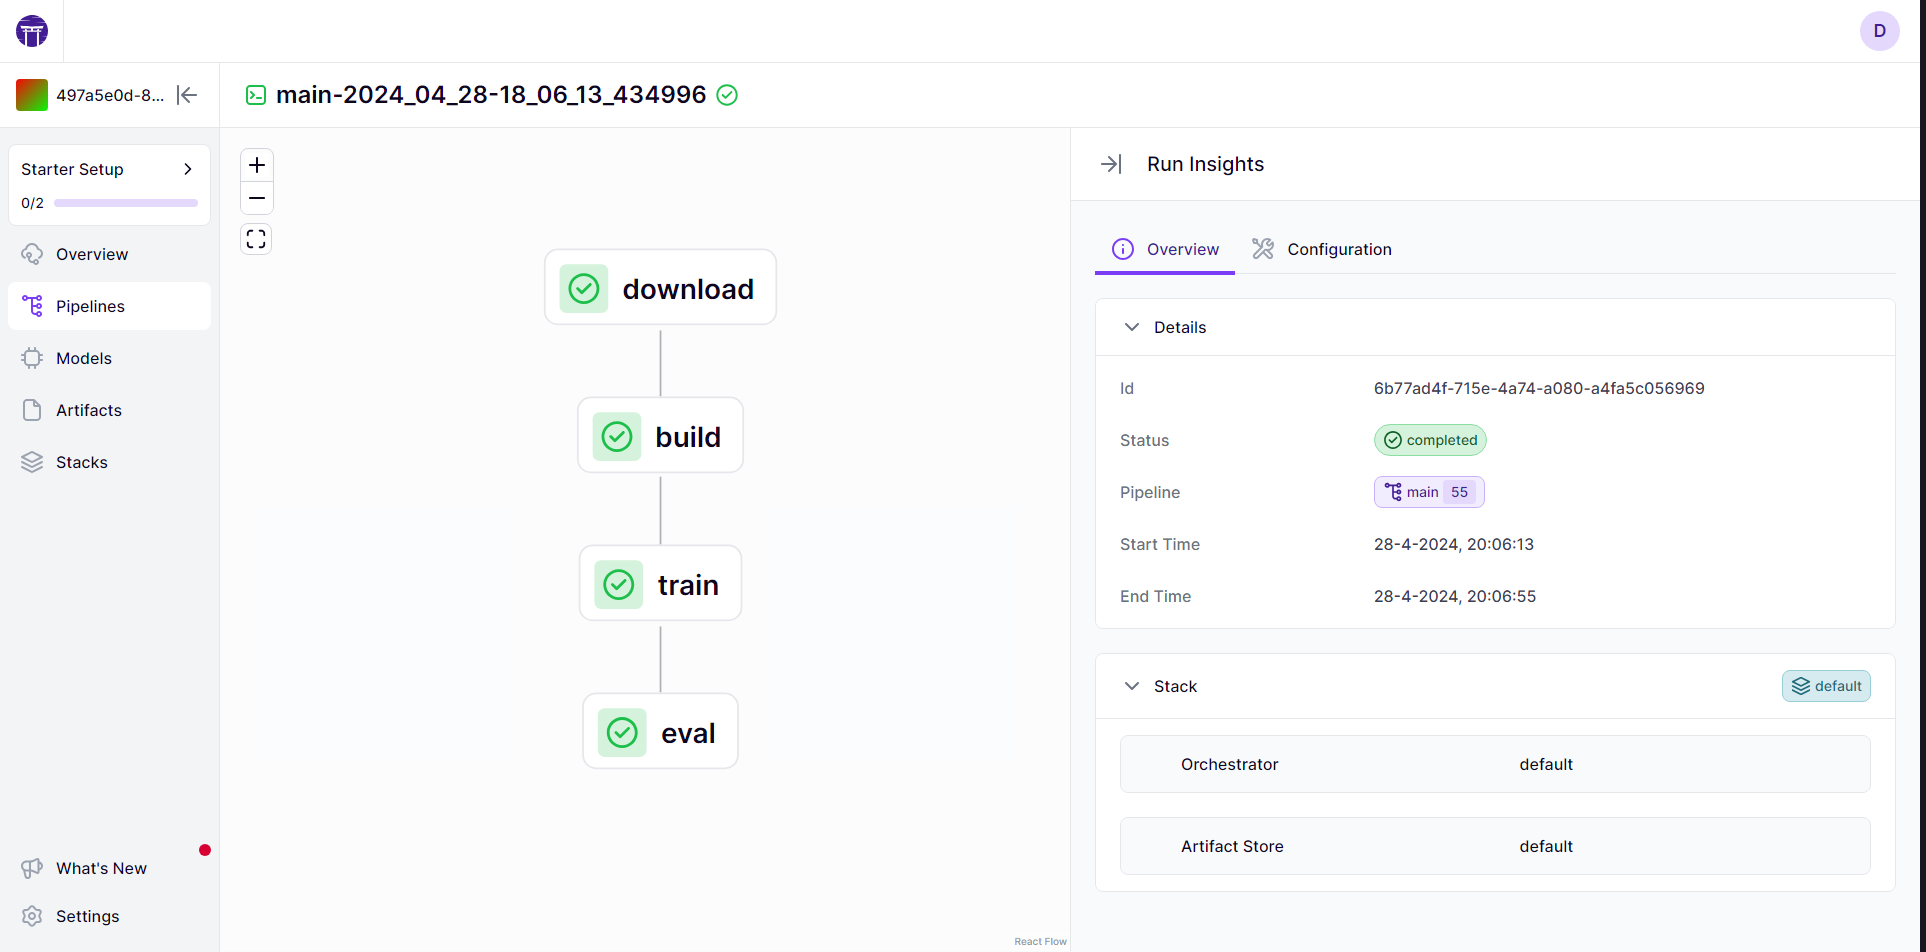
\includegraphics[width=0.9\linewidth]{graphics/ZenML_Pipeline_Flow.PNG}
    \caption{ZenML pipeline flow}
    \label{fig:ZenML_Pipeline_Flow}
\end{figure}
\subsection{Problemen}

\subsection{Cloud}
Prefect heeft een concept genaamd \textit{Stacks}. ZenML is net geupgrade naar versie 0.57.0 waardoor heel het dashboard veranderd is en nog in ontwikkeling is.
Deze pagina is dus nog niet beschikbaar maar de functionaliteit kan al via de command-line-interface (CLI) gebruikt worden.

Als deze pagina beschikbaar


\section{Dagster}
Deze Proof of Concept zal gebruik maken van Dagster en MLFlow
\subsection{Installatie}
De installatie van Dagster verloopt via de package manager \texttt{pip}. Dagster ondersteunt Python versies 3.8 tot 3.12 en kan met het volgende commando worden geïnstalleerd:
\begin{minted}[frame=lines,breaklines,linenos]{bash}
    pip install dagster dagster-webserver
\end{minted}
Om Dagster te installeren op een Mac met een Apple Silicon chip moet het volgende commando gebruikt worden:
\begin{minted}[frame=lines,breaklines,linenos]{bash}
    pip install dagster dagster-webserver --find-links=https://github.com/dagster-io/build-grpcio/wiki/Wheels
\end{minted}
Na het installeren van Dagster kan er een project aangemaakt worden via de terminal met het volgende commando:
\begin{minted}[frame=lines,breaklines,linenos]{bash}
    dagster project scaffold --name my-dagster-project
\end{minted}
Het bovenstaande commando maakt een mapstructuur aan met ruimte voor de pipeline en andere bestanden voor het opzetten van een project in Dagster. Er is ook een parameter \textit{name} die de naam van het project definieert.
Na het aanmaken van het project kan de webserver worden opgestart. Dit kan met het volgende commando. Voordat je het commando uitvoert, moet je echter naar de map navigeren waar het Dagster-project zich bevindt:
\begin{minted}[frame=lines,breaklines,linenos]{bash}
    dagster dev
\end{minted}
\subsection{Dashboard}
Na het opstarten van de webserver kun je via het webadres in de terminal naar het Dagster-dashboard gaan. Het Dagster-dashboard is een omgeving waarin alle pipelines worden beheerd.
Het dashboard ziet eruit zoals in figuur~\ref{fig:Dagser_assets}
\begin{figure}
    \centering
    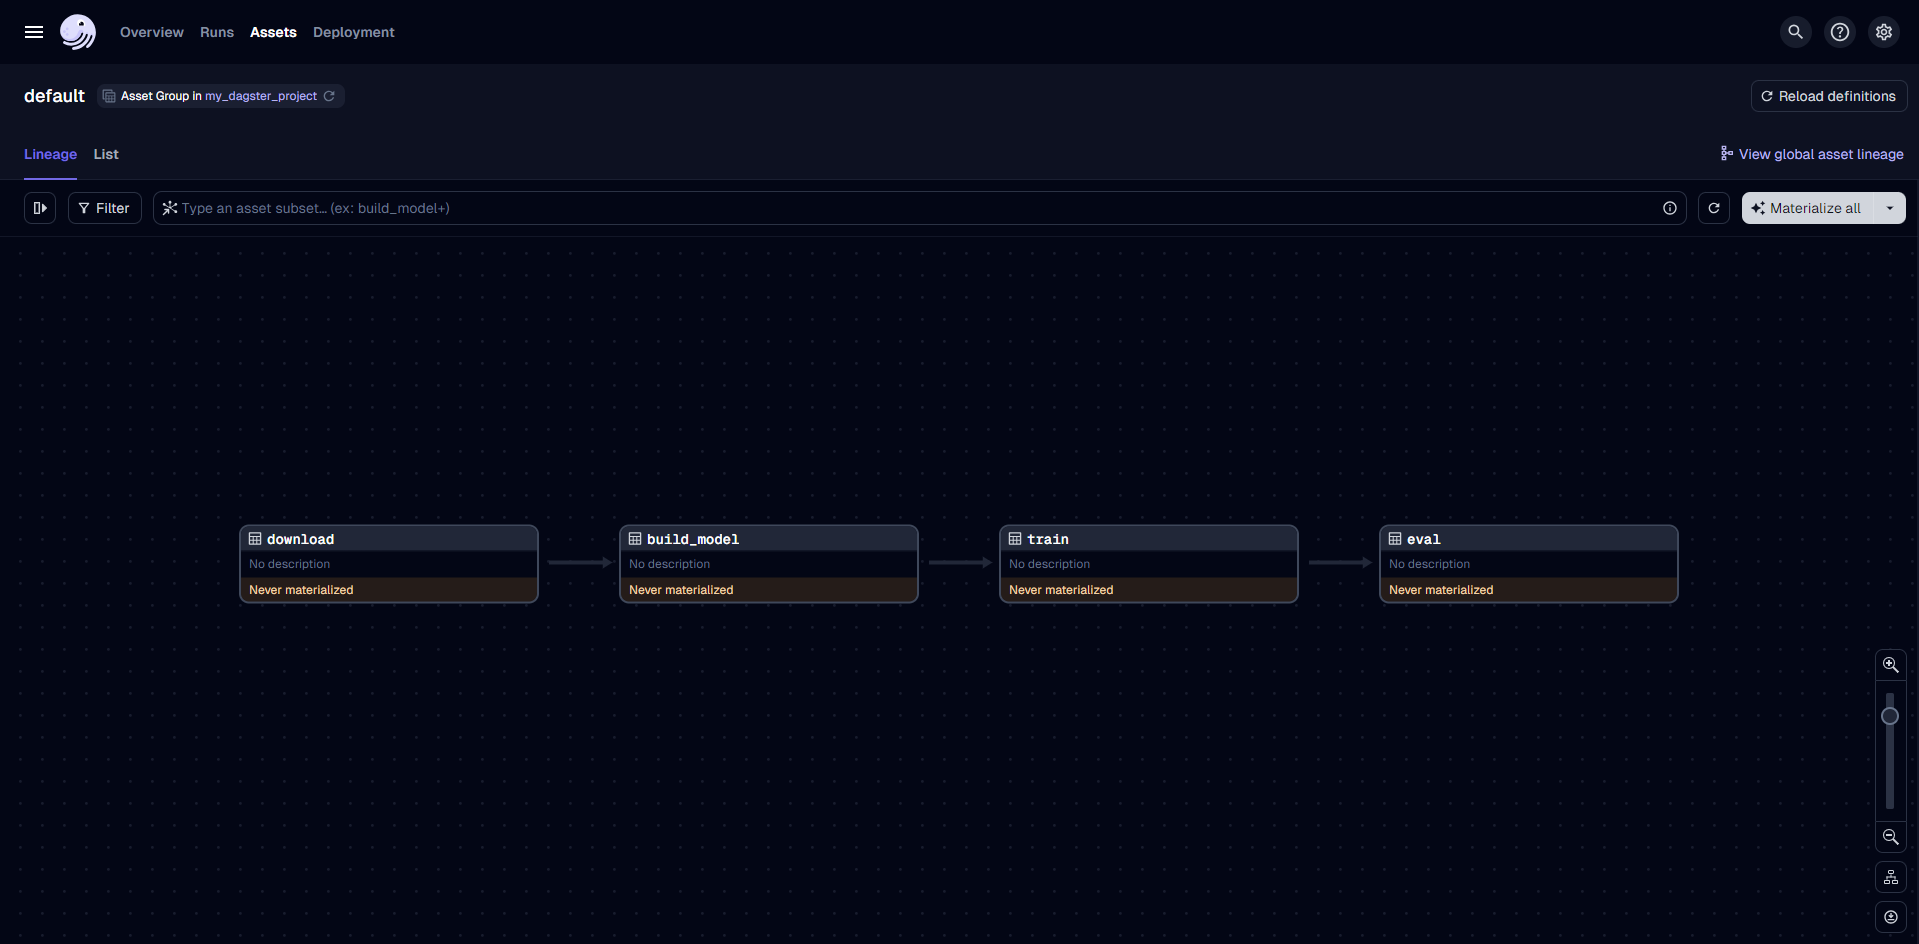
\includegraphics[width=0.9\linewidth]{graphics/Dagster_Assets.PNG}
    \caption{Dagster assets overview}
    \label{fig:Dagser_assets}
\end{figure}
Standaard wordt je naar de asset pagina van Dagster verwijst als je op de link de terminal klikt zoals in figuur~\ref{fig:Dagser_assets}
\subsection{Uitvoering}

\subsection{Pipeline}
\subsection{Problemen}
Tijdens het uitvoeren van de Proof of Concept zijn er enkele problemen opgedoken.
Het eerste probleem was dat Dagster verschillende data types niet ondersteund als parameters voor \textit{assets} waardoor het model niet meegegeven kon worden naar de opeenvolgende functie. Om dit op te lossen is het model lokaal opgeslagen om in de opeenvogende functie deze terug in te lezen en dit voor elke opeenvolgende functie.
\subsection{Cloud}
